\documentclass[12pt]{article}
\usepackage[utf8]{inputenc}
\usepackage[a4paper, margin=2cm]{geometry}
\usepackage[T1]{fontenc}
\usepackage{graphicx}
\usepackage{geometry}
\usepackage{amsmath}
\usepackage{amsfonts}
\usepackage{amssymb}
\usepackage{booktabs}
\usepackage{hyperref}
\usepackage{fancyhdr}
\usepackage{float}
\usepackage{ulem}
\usepackage{xeCJK}
\usepackage{listings}
\usepackage{xcolor}
\usepackage{indentfirst}
\setmainfont{Times New Roman}
\setCJKmonofont[BoldFont=SimHei, AutoFakeBold=true]{SimSun}
\lstset{
    basicstyle=\ttfamily\small,
    commentstyle=\color{gray},
    keywordstyle=\color{blue},
    stringstyle=\color{red},
    numberstyle=\tiny\color{gray},
    breaklines=true,
    captionpos=b,
    keepspaces=true,
    numbers=left,
    numbersep=5pt,
    showspaces=false,
    showstringspaces=false,
    showtabs=false,
    tabsize=2,
    frame=single,
    language=[x86masm]Assembler
}

\begin{document}
\thispagestyle{empty}

\begin{center}
    \vspace*{2cm}
    
    \Huge \textbf{2023-2024学年春季学期} \\
    \vspace{2cm}
    
    \Huge \textbf{《汇编语言程序设计》} \\
    \vspace{4cm}
    
    \large 评分：\underline{\hspace{4cm}} \\
    \vspace{6cm}
    
    \begin{tabular}{rl}
        \Large 学\hspace{2em}院： & \Large \underline{\makebox[12em][l]{\quad 计算机科学与工程学院}} \\
        \Large 专\hspace{2em}业： & \Large \underline{\makebox[12em][l]{\quad 计算机科学与技术}} \\
        \Large 班\hspace{2em}级： & \Large \underline{\makebox[12em][l]{\quad 计算机2204班}} \\
        \Large 姓\hspace{2em}名： & \Large \underline{\makebox[12em][l]{\quad 李俊洁}} \\
        \Large 学\hspace{2em}号： & \Large \underline{\makebox[12em][l]{\quad 20225443}} \\
        \Large 任课教师：         & \Large \underline{\makebox[12em][l]{\quad 刘思宇、柳秀梅}} \\
    \end{tabular}
    \vfill
\end{center}
\newpage

\section{实验目的}
本实验旨在通过汇编语言编程，实现基本的算术运算（加、减、乘、除）功能，加深对汇编语言在实际应用中的运算处理能力的理解。
通过键盘输入数据和屏幕输出结果的方式，让学生深入学习汇编语言与硬件交互的基本方法，包括使用中断服务进行输入输出操作。
实验通过编写和测试一个简单的算术运算程序，帮助学生掌握汇编语言中的数据转换、条件判断和分支处理等关键编程技能。

具体学习目标包括：
\begin{itemize}
    \item 理解和应用汇编语言进行基本的算术运算。
    \item 学习使用DOS中断调用来实现程序的输入和输出。
    \item 掌握如何在汇编语言程序中处理用户输入的数据，并据此执行相应的运算。
    \item 提升调试和错误处理能力，通过实际编码实践解决编程中遇到的问题。
    \item 加强对程序控制流的理解，包括条件分支和跳转等。
\end{itemize}

\section{实验要求}
遵循以下详细要求来完成实验，实验要求如下：
\begin{itemize}
    \item 程序必须能从键盘接收输入，包括两个一位十进制数字和一个运算符（加、减、乘、除）。结果必须在屏幕上正确显示，包括处理和显示可能的负数结果。
    \item 程序需实现加、减、乘、除四种基本运算。对于除法操作，需添加除数为零时的错误处理机制，防止程序异常中断。
    \item 程序应具有清晰的结构，合理的模块化设计。各算术操作应通过不同的程序段实现，以提高代码的可读性和可维护性。
    \item 使用适当的DOS中断（如INT 21h）来实现输入输出功能，深入理解中断的使用方式和作用。
    \item 输入的数据必须进行有效性验证，确保输入数据为有效的一位十进制数字，运算符也必须是指定的四种操作之一。
    \item 提交的源代码必须包含充分的注释，解释每个部分的功能和关键逻辑。实验报告应详细记录程序的设计思路、实现过程以及遇到的问题和解决方案。
\end{itemize}

通过满足上述要求能展示对汇编语言编程及其在实际应用中处理输入输出和基本运算的能力。
此外，这些要求还旨在帮助学生学习如何结构化编写程序，提高编程效率和质量。
\section{实验内容}
编写一个能实现两个一位十进制数据的加、减、乘、除功能的程序。
\begin{itemize}
    \item 原始数据从键盘输入。
    \item 结果在显示器上显示。
\end{itemize}
\section{源程序}
    \begin{lstlisting}[caption={汇编源代码}, label=lst:asm2]
dseg   segment
    data1       db 0
    data2       db 0
    operation   db 0
dseg   ends

sseg    segment  stack
    stack   db  100h  dup  (?)
sseg    ends

cseg    segment
    assume cs:cseg, ds:dseg, ss:sseg
start:
    mov  ax, dseg               ; 初始化
    mov  ds, ax
    mov  ax, sseg
    mov  ss, ax
    mov  sp, 100h

    mov ah, 01h                 ; 设置功能号为01h（读取字符）
    int 21h                     ; 调用中断读取一个字符到al
    sub al, 30h                 ; 将读取的字符转换为数字
    mov data1, al               ; 将读取的字符存储到data1

    mov ah, 01h                 ; 设置功能号为01h（读取字符）
    int 21h                     ; 调用中断读取一个字符到al
    mov operation, al           ; 将读取的字符存储到operation

    mov ah, 01h                 ; 设置功能号为01h（读取字符）
    int 21h                     ; 调用中断读取一个字符到al
    sub al, 30h                 ; 将读取的字符转换为数字
    mov data2, al               ; 存储到data2

    mov al, operation
    cmp al, '+'
    je  my_add
    cmp al, '-'
    je  my_sub
    cmp al, '*'
    je  my_mul
    cmp al, '/'
    je  my_div
    jmp end_program

my_add:
    mov  al, data1
    add  al, data2
    jmp  return

my_sub:
    mov  al, data1
    sub  al, data2
    jmp  return

my_mul:
    mov  al, data1
    mul  data2
    jmp  return

my_div:
    mov  al, data2                ; 确保除数不为0
    add  al, 0
    jz   end_program

    xor  ax, ax
    mov  al, data1
    div  data2
    jmp  return

return:
    mov bl, al                   ; 将结果存储到bl
    mov dl, ' '                  ; 显示空格
    mov ah, 02h
    int 21h

    mov  dl, bl                   ; 显示结果
    add  dl, 0
    jns  is_positive
    mov  dl, '-'                  ; 显示负号
    mov  ah, 02h
    int  21h
    neg  bl

is_positive:
    xor  ax, ax
    mov  al, bl
    mov  bl, 10                   ; 结果可能比10更大，因此要转换为十进制输出。
    div  bl                       ; ah是余数，al是商
    mov  dl, al                   ; 商为十位数。
    mov  dh, ah                   ; 余数为个位

    add  al, 0
    jz   is_zero
    add  dl, 30h
    mov  ah, 02h                  ; 输出商
    int  21h

is_zero:
    mov  dl, dh
    add  dl, 30h                  ; 输出余数
    mov  ah, 02h
    int  21h

end_program:
    mov  ah, 4ch                 ; 结束程序
    int  21h

cseg    ends
    end  start

    \end{lstlisting}

\section{运行结果}
    \subsection{显示结果}
    三种数据时分别的显示结果：

    加：
    \begin{center}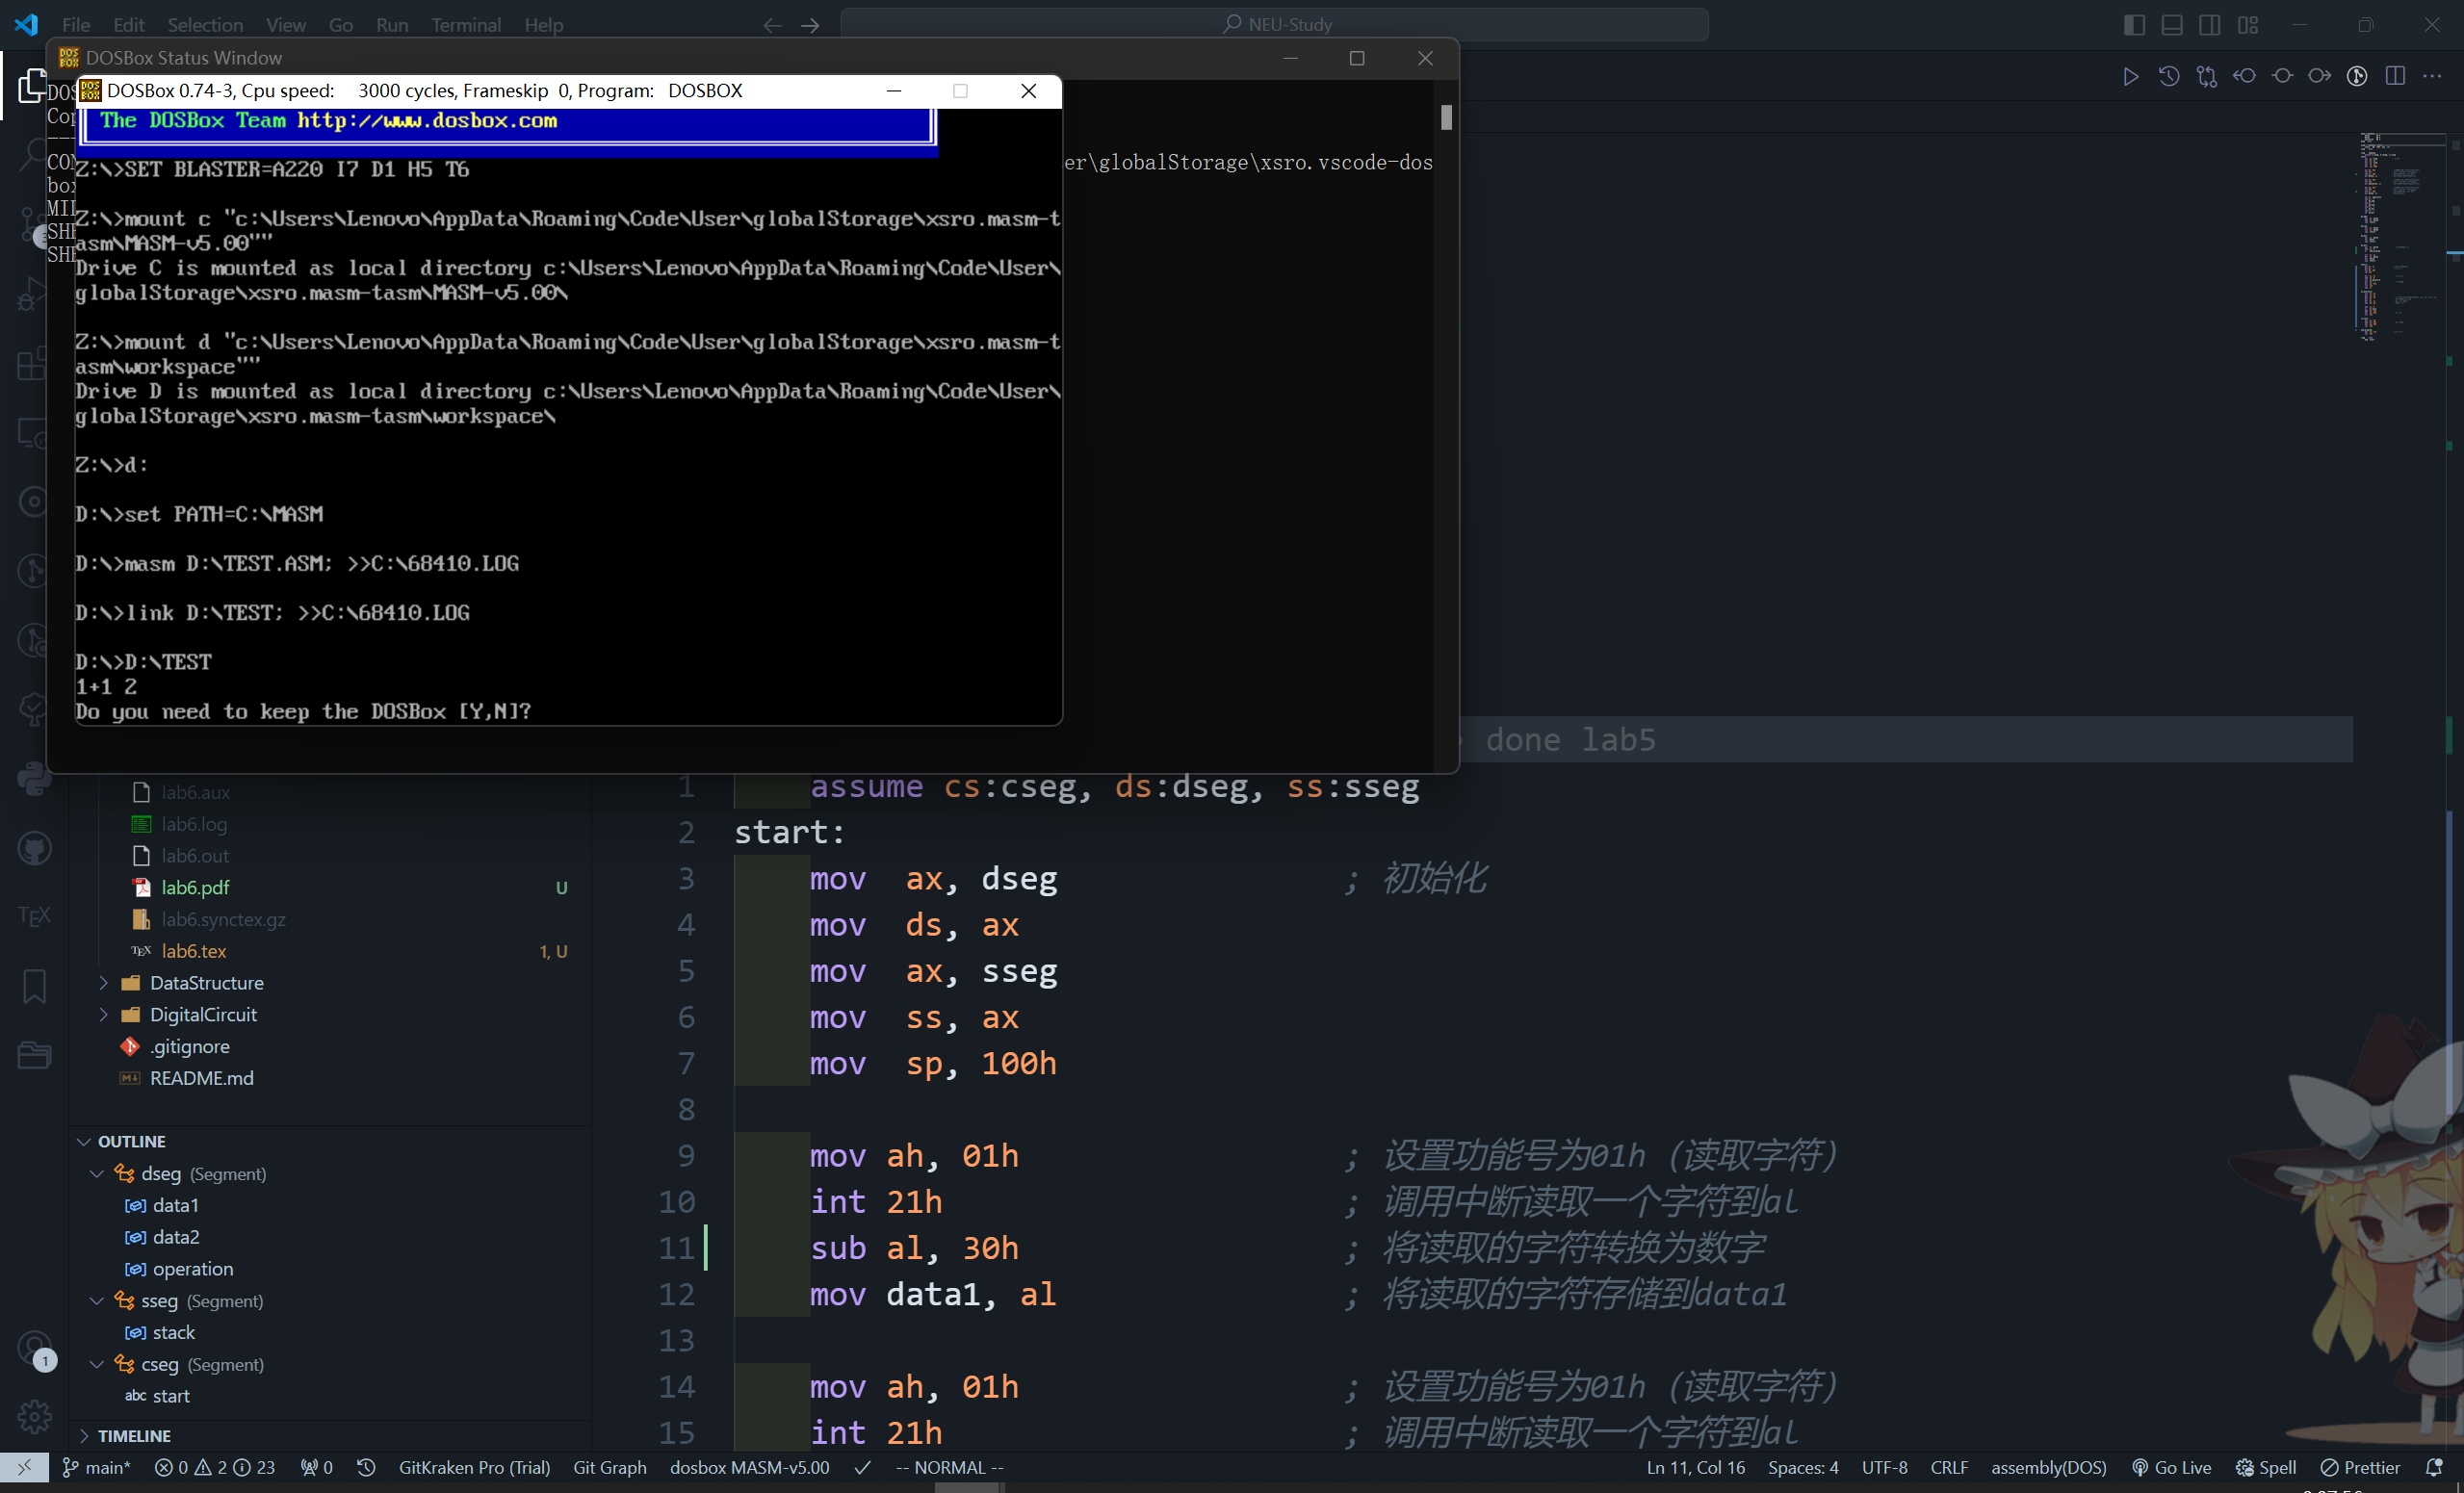
\includegraphics[width=1\textwidth]{image/AL_53.png}\end{center}
    \begin{center}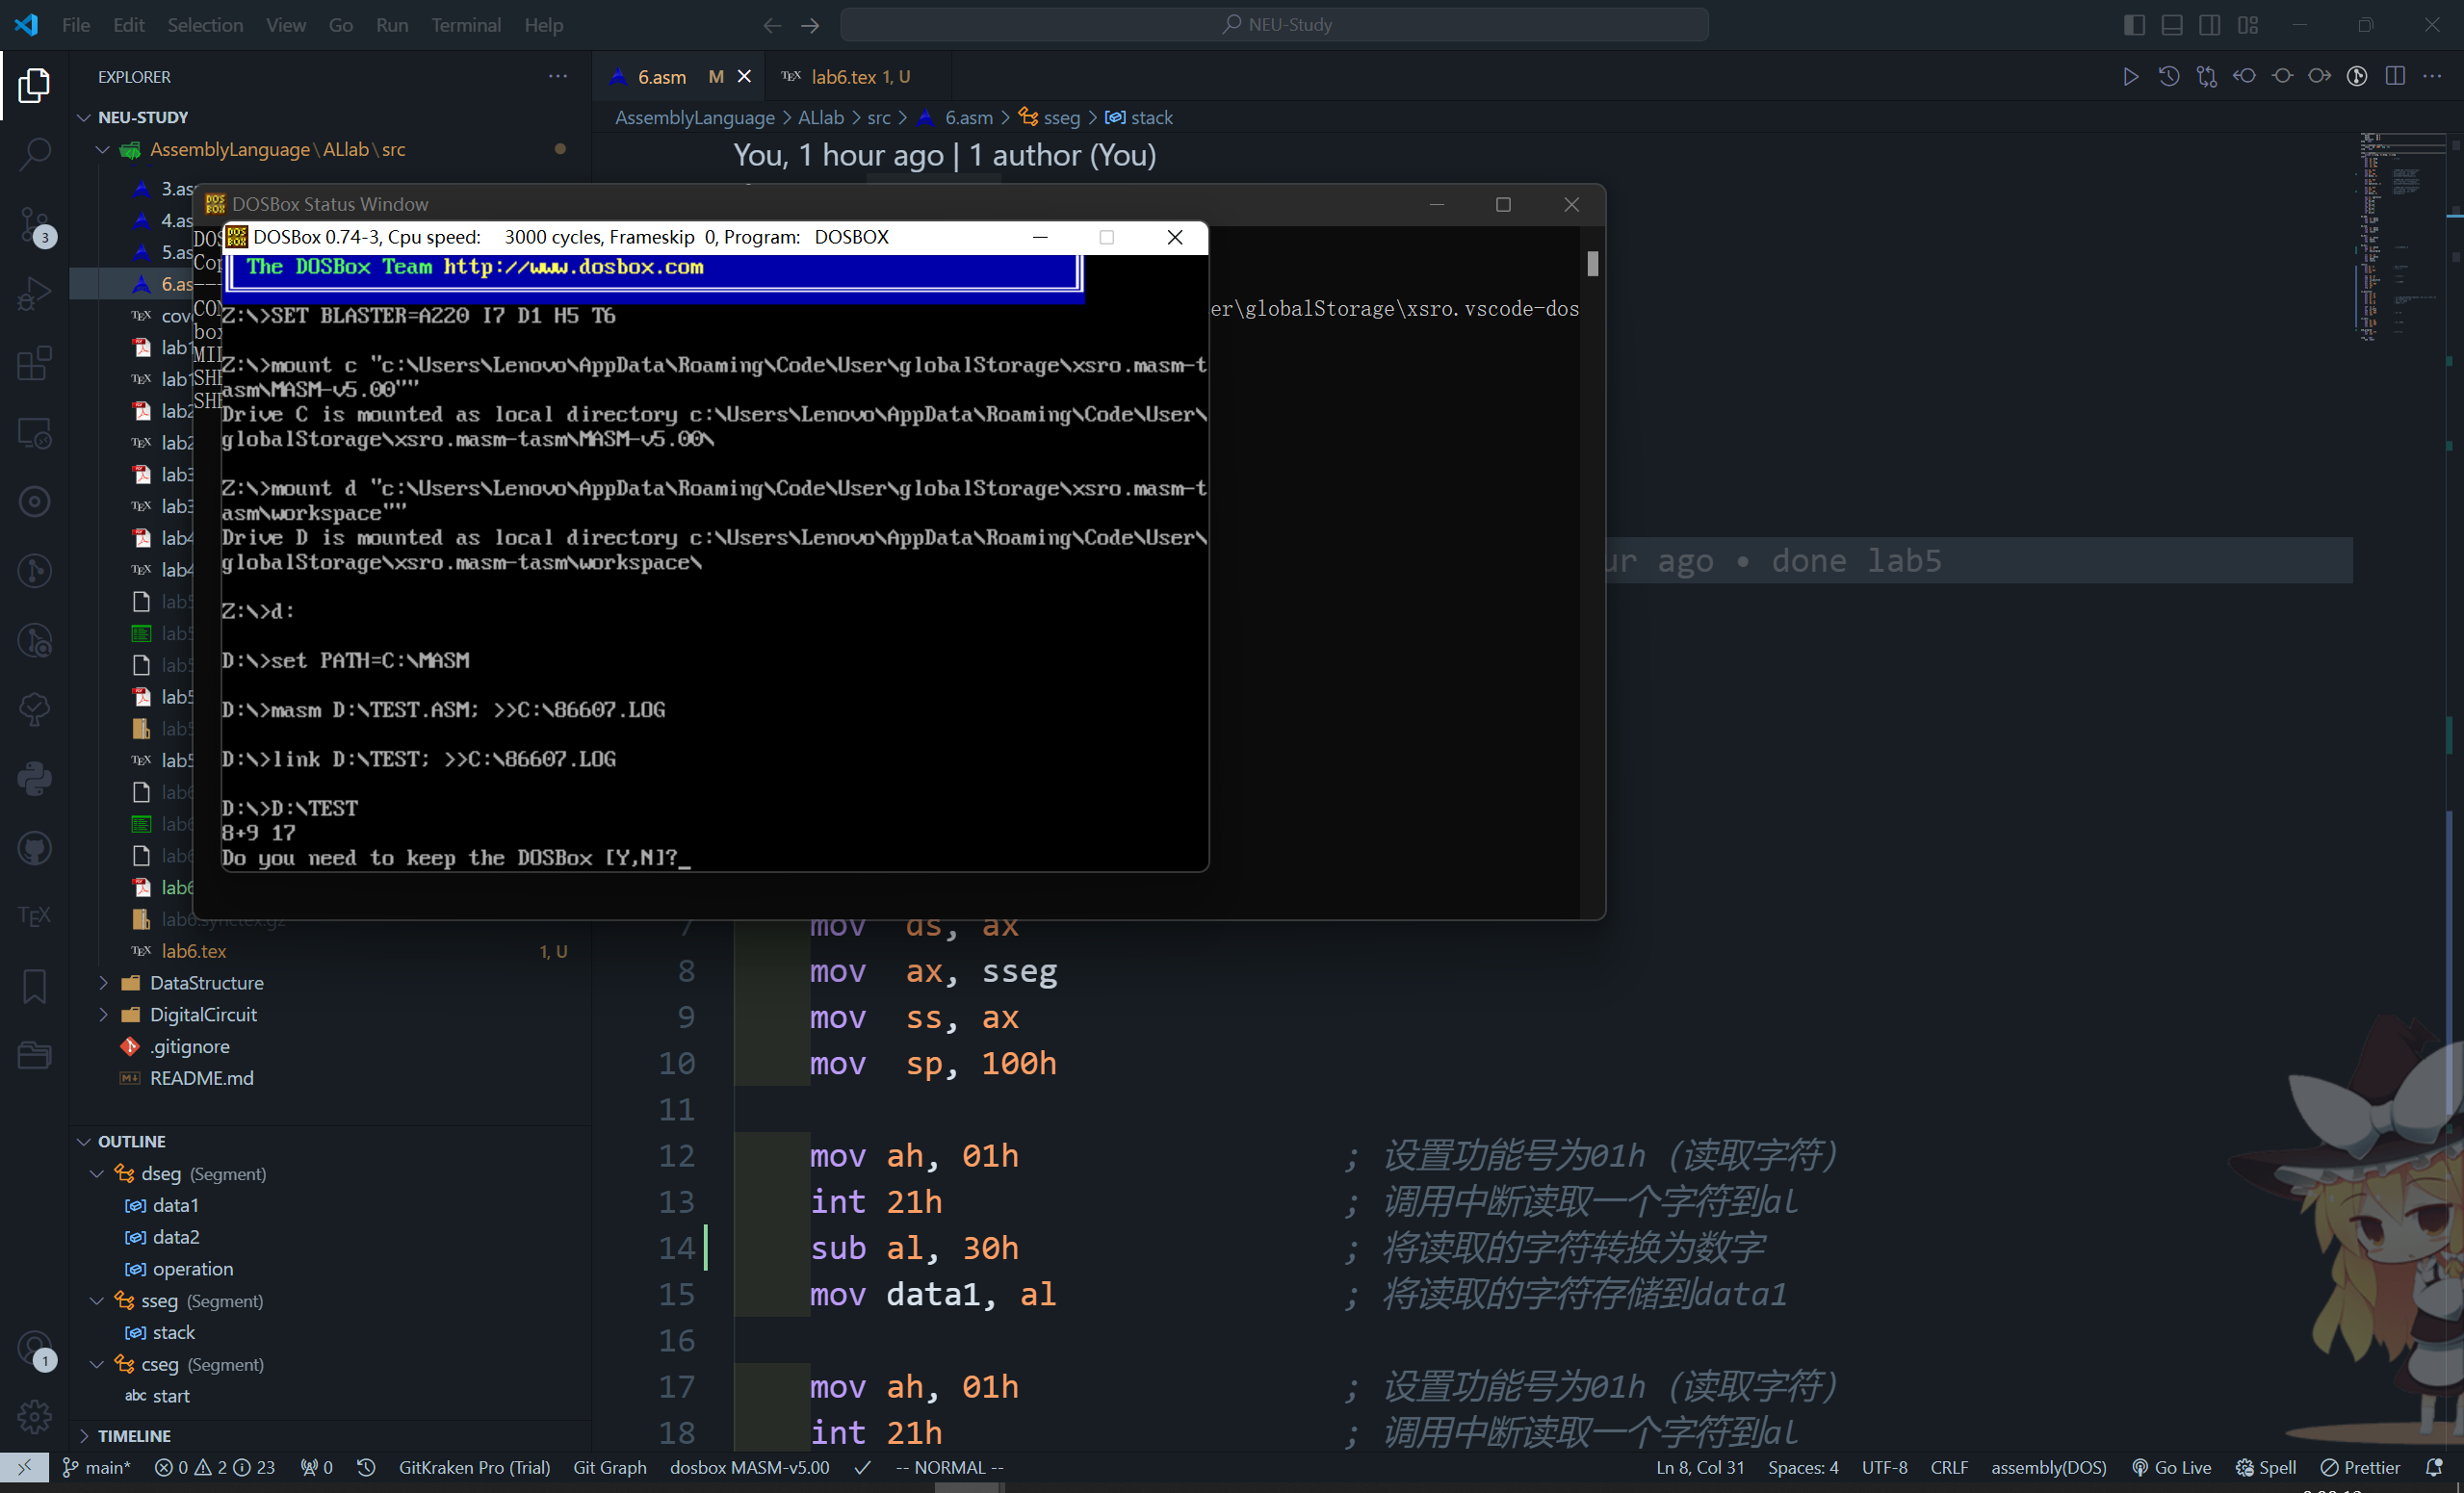
\includegraphics[width=1\textwidth]{image/AL_54.png}\end{center}
    减：
    \begin{center}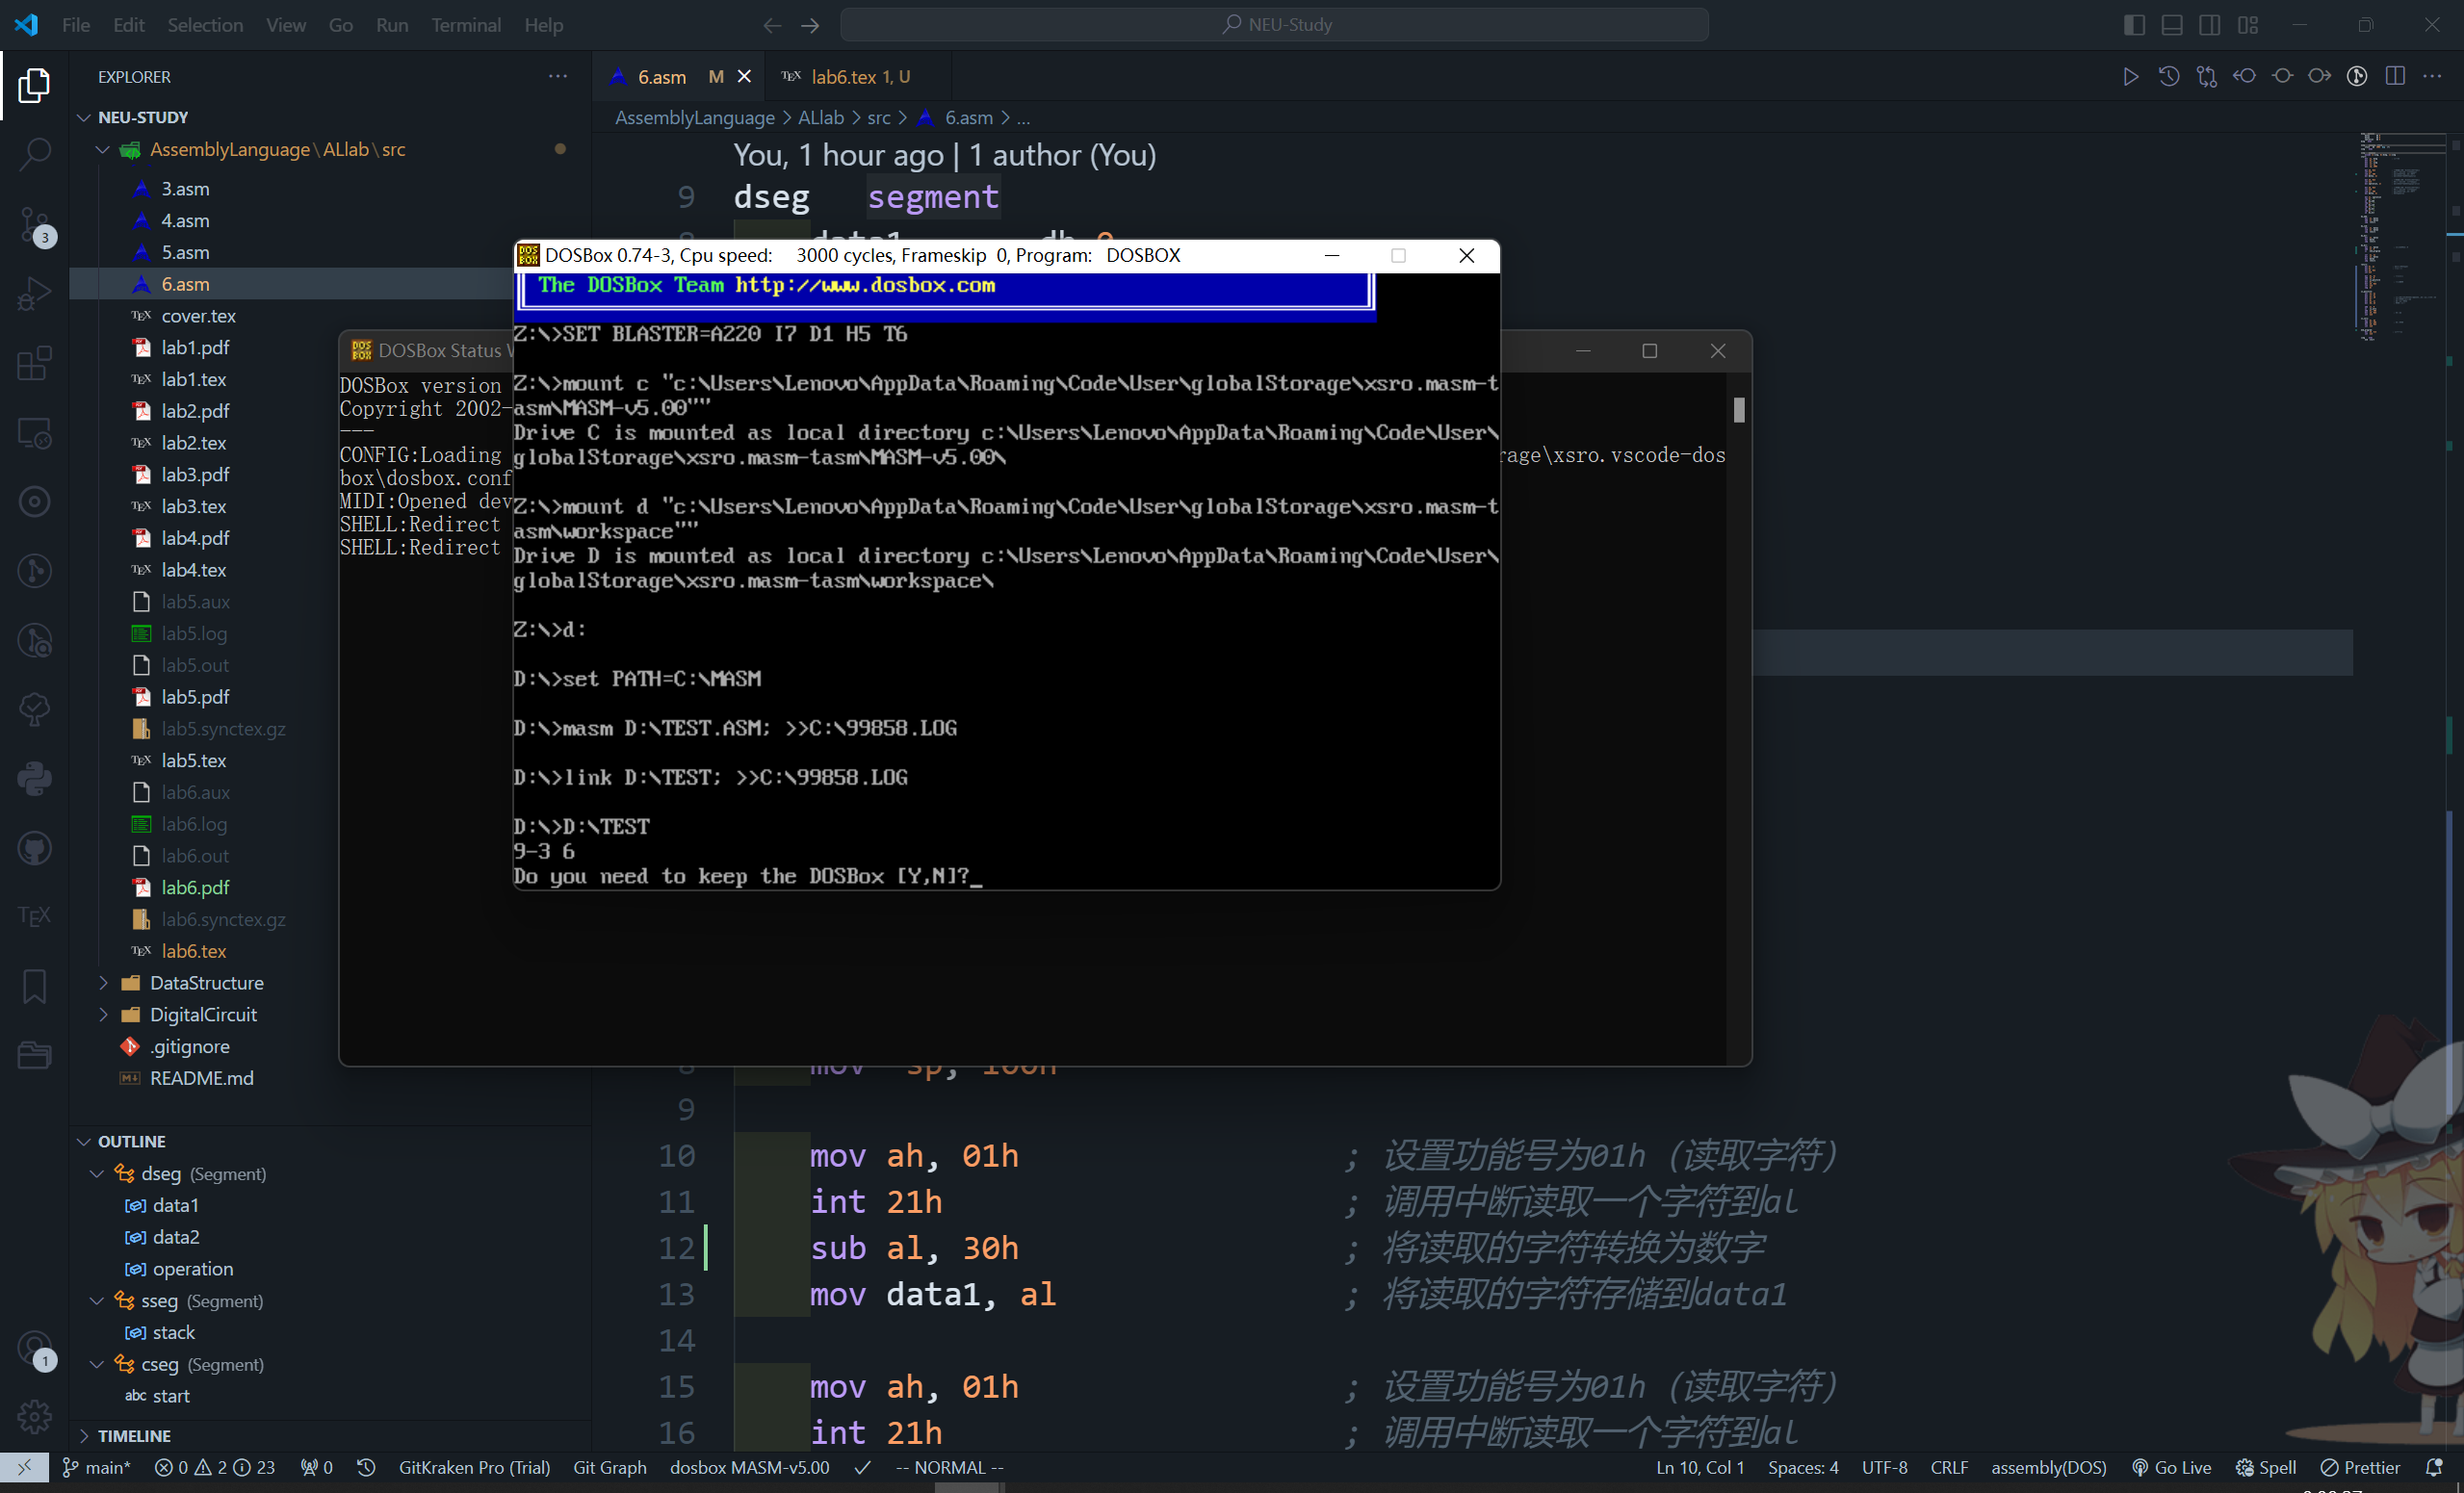
\includegraphics[width=1\textwidth]{image/AL_55.png}\end{center}
    \begin{center}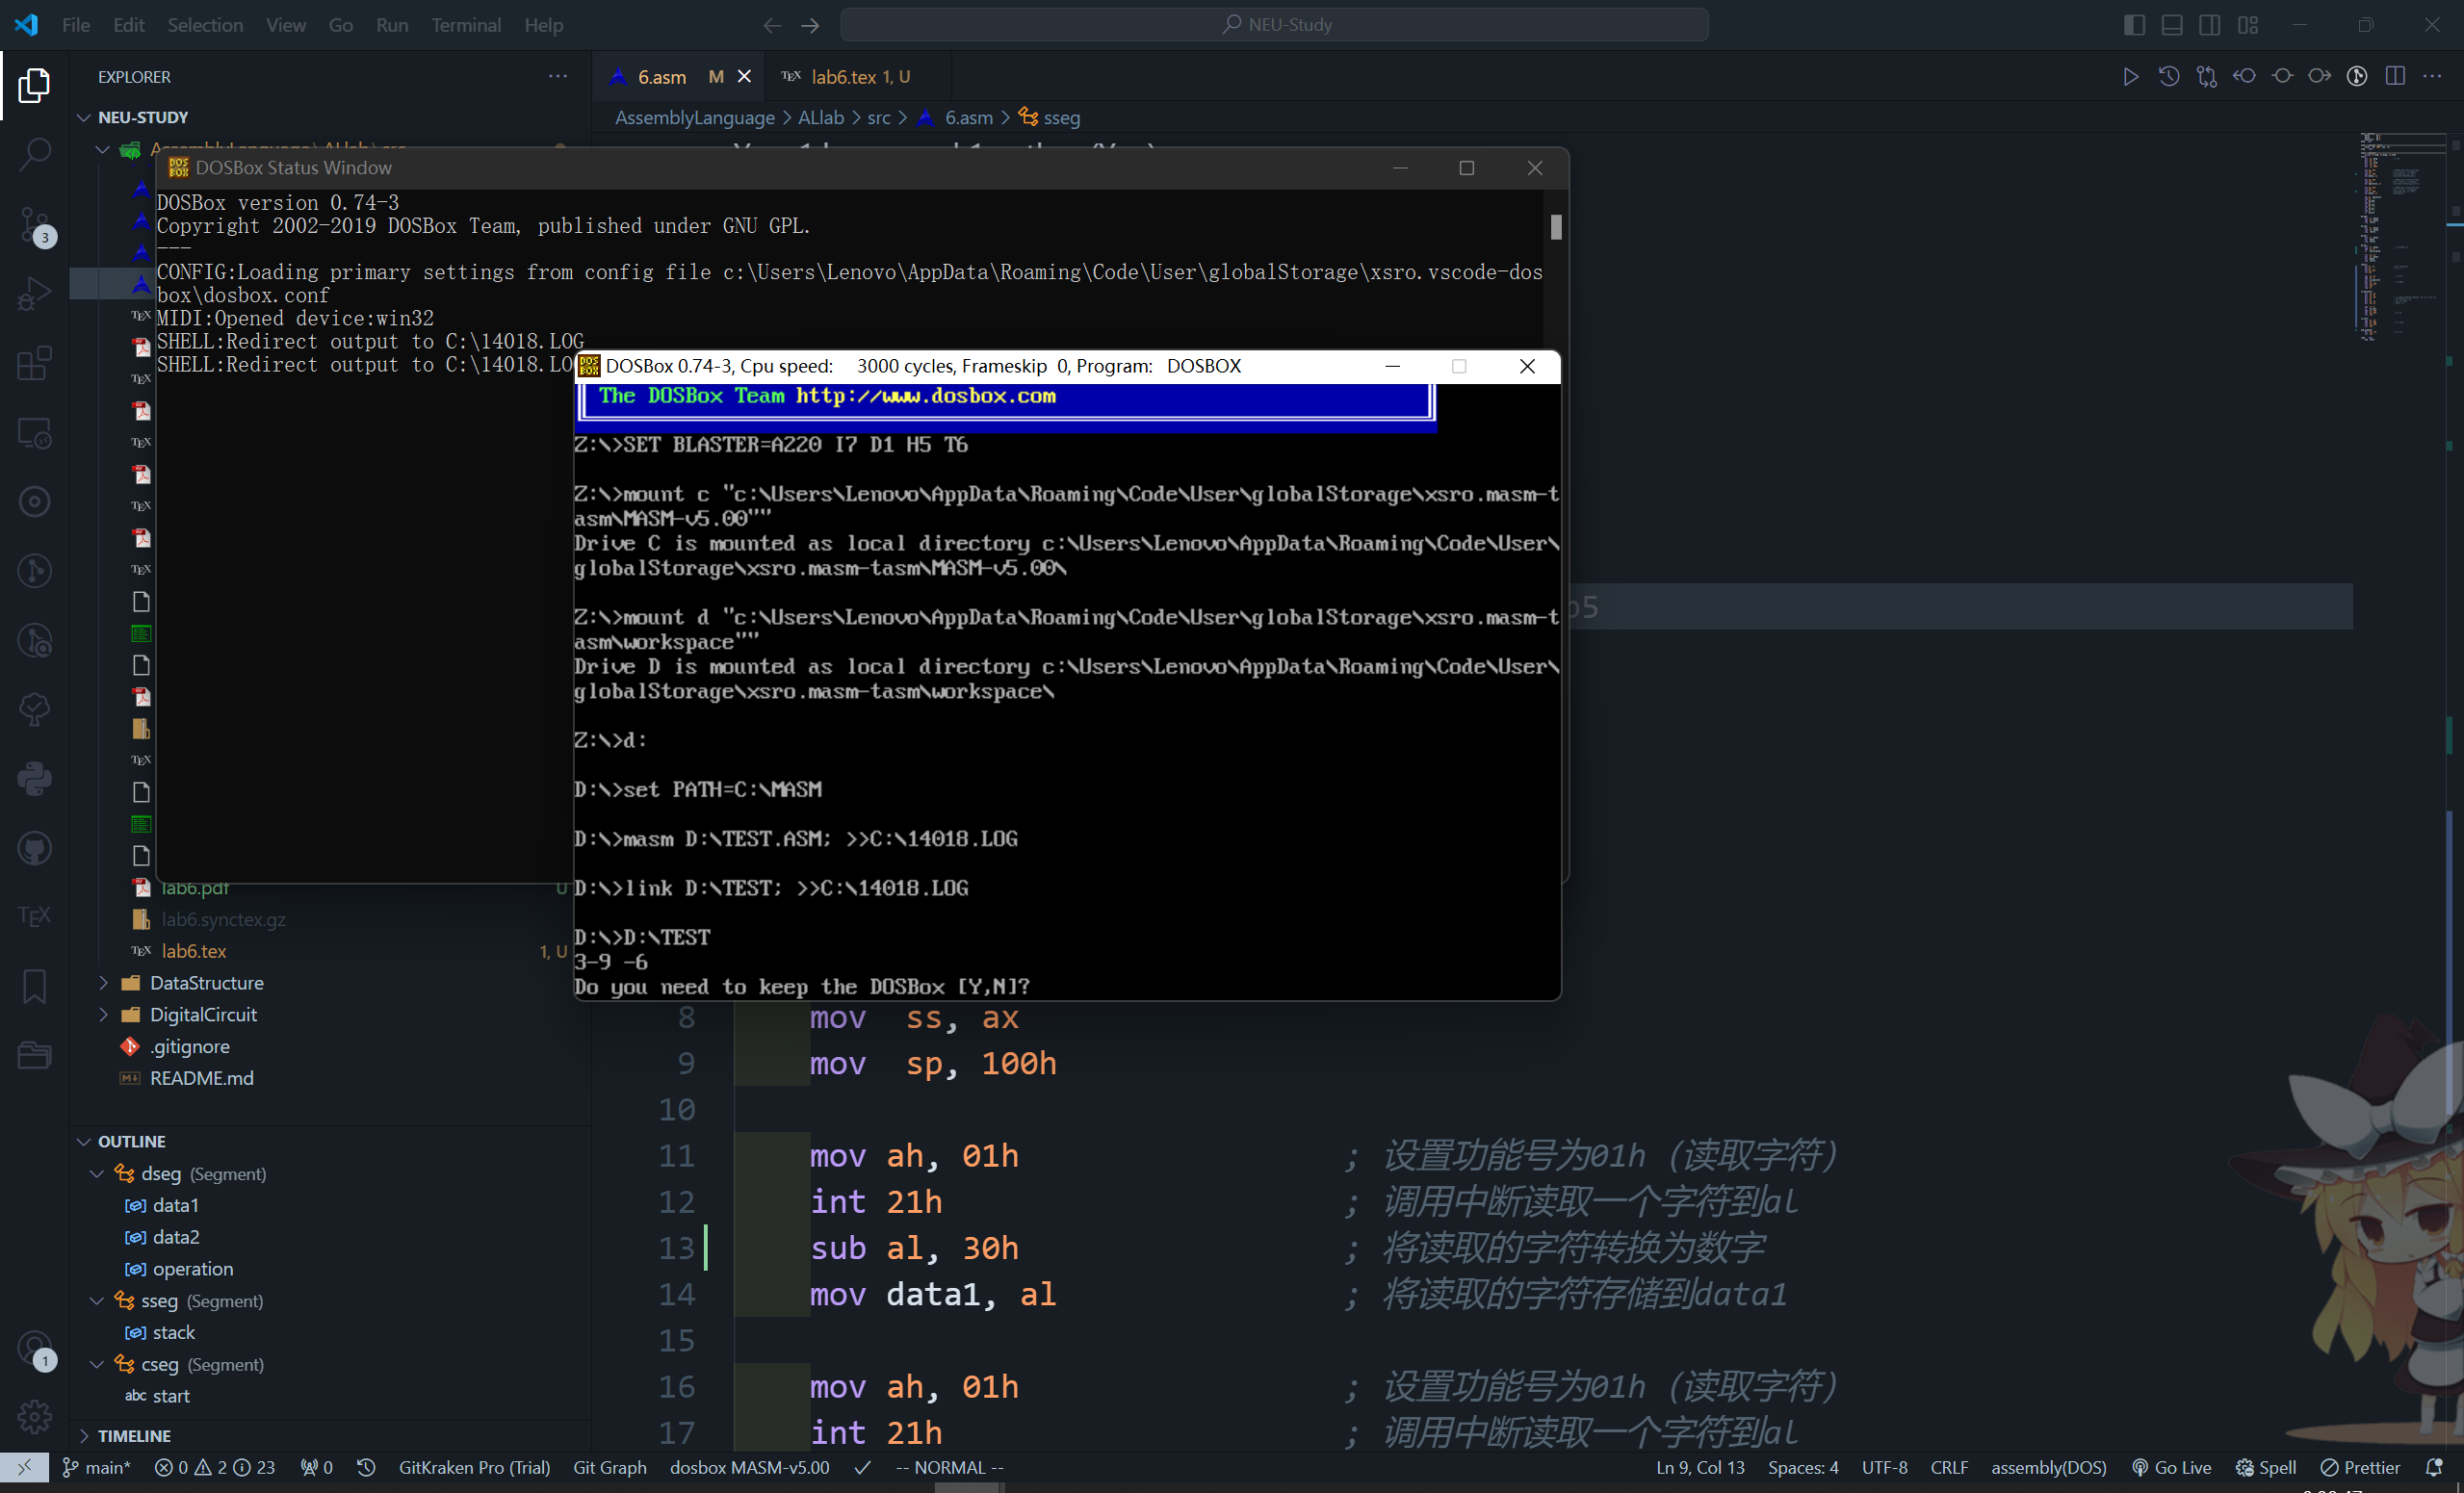
\includegraphics[width=1\textwidth]{image/AL_56.png}\end{center}
    乘：
    \begin{center}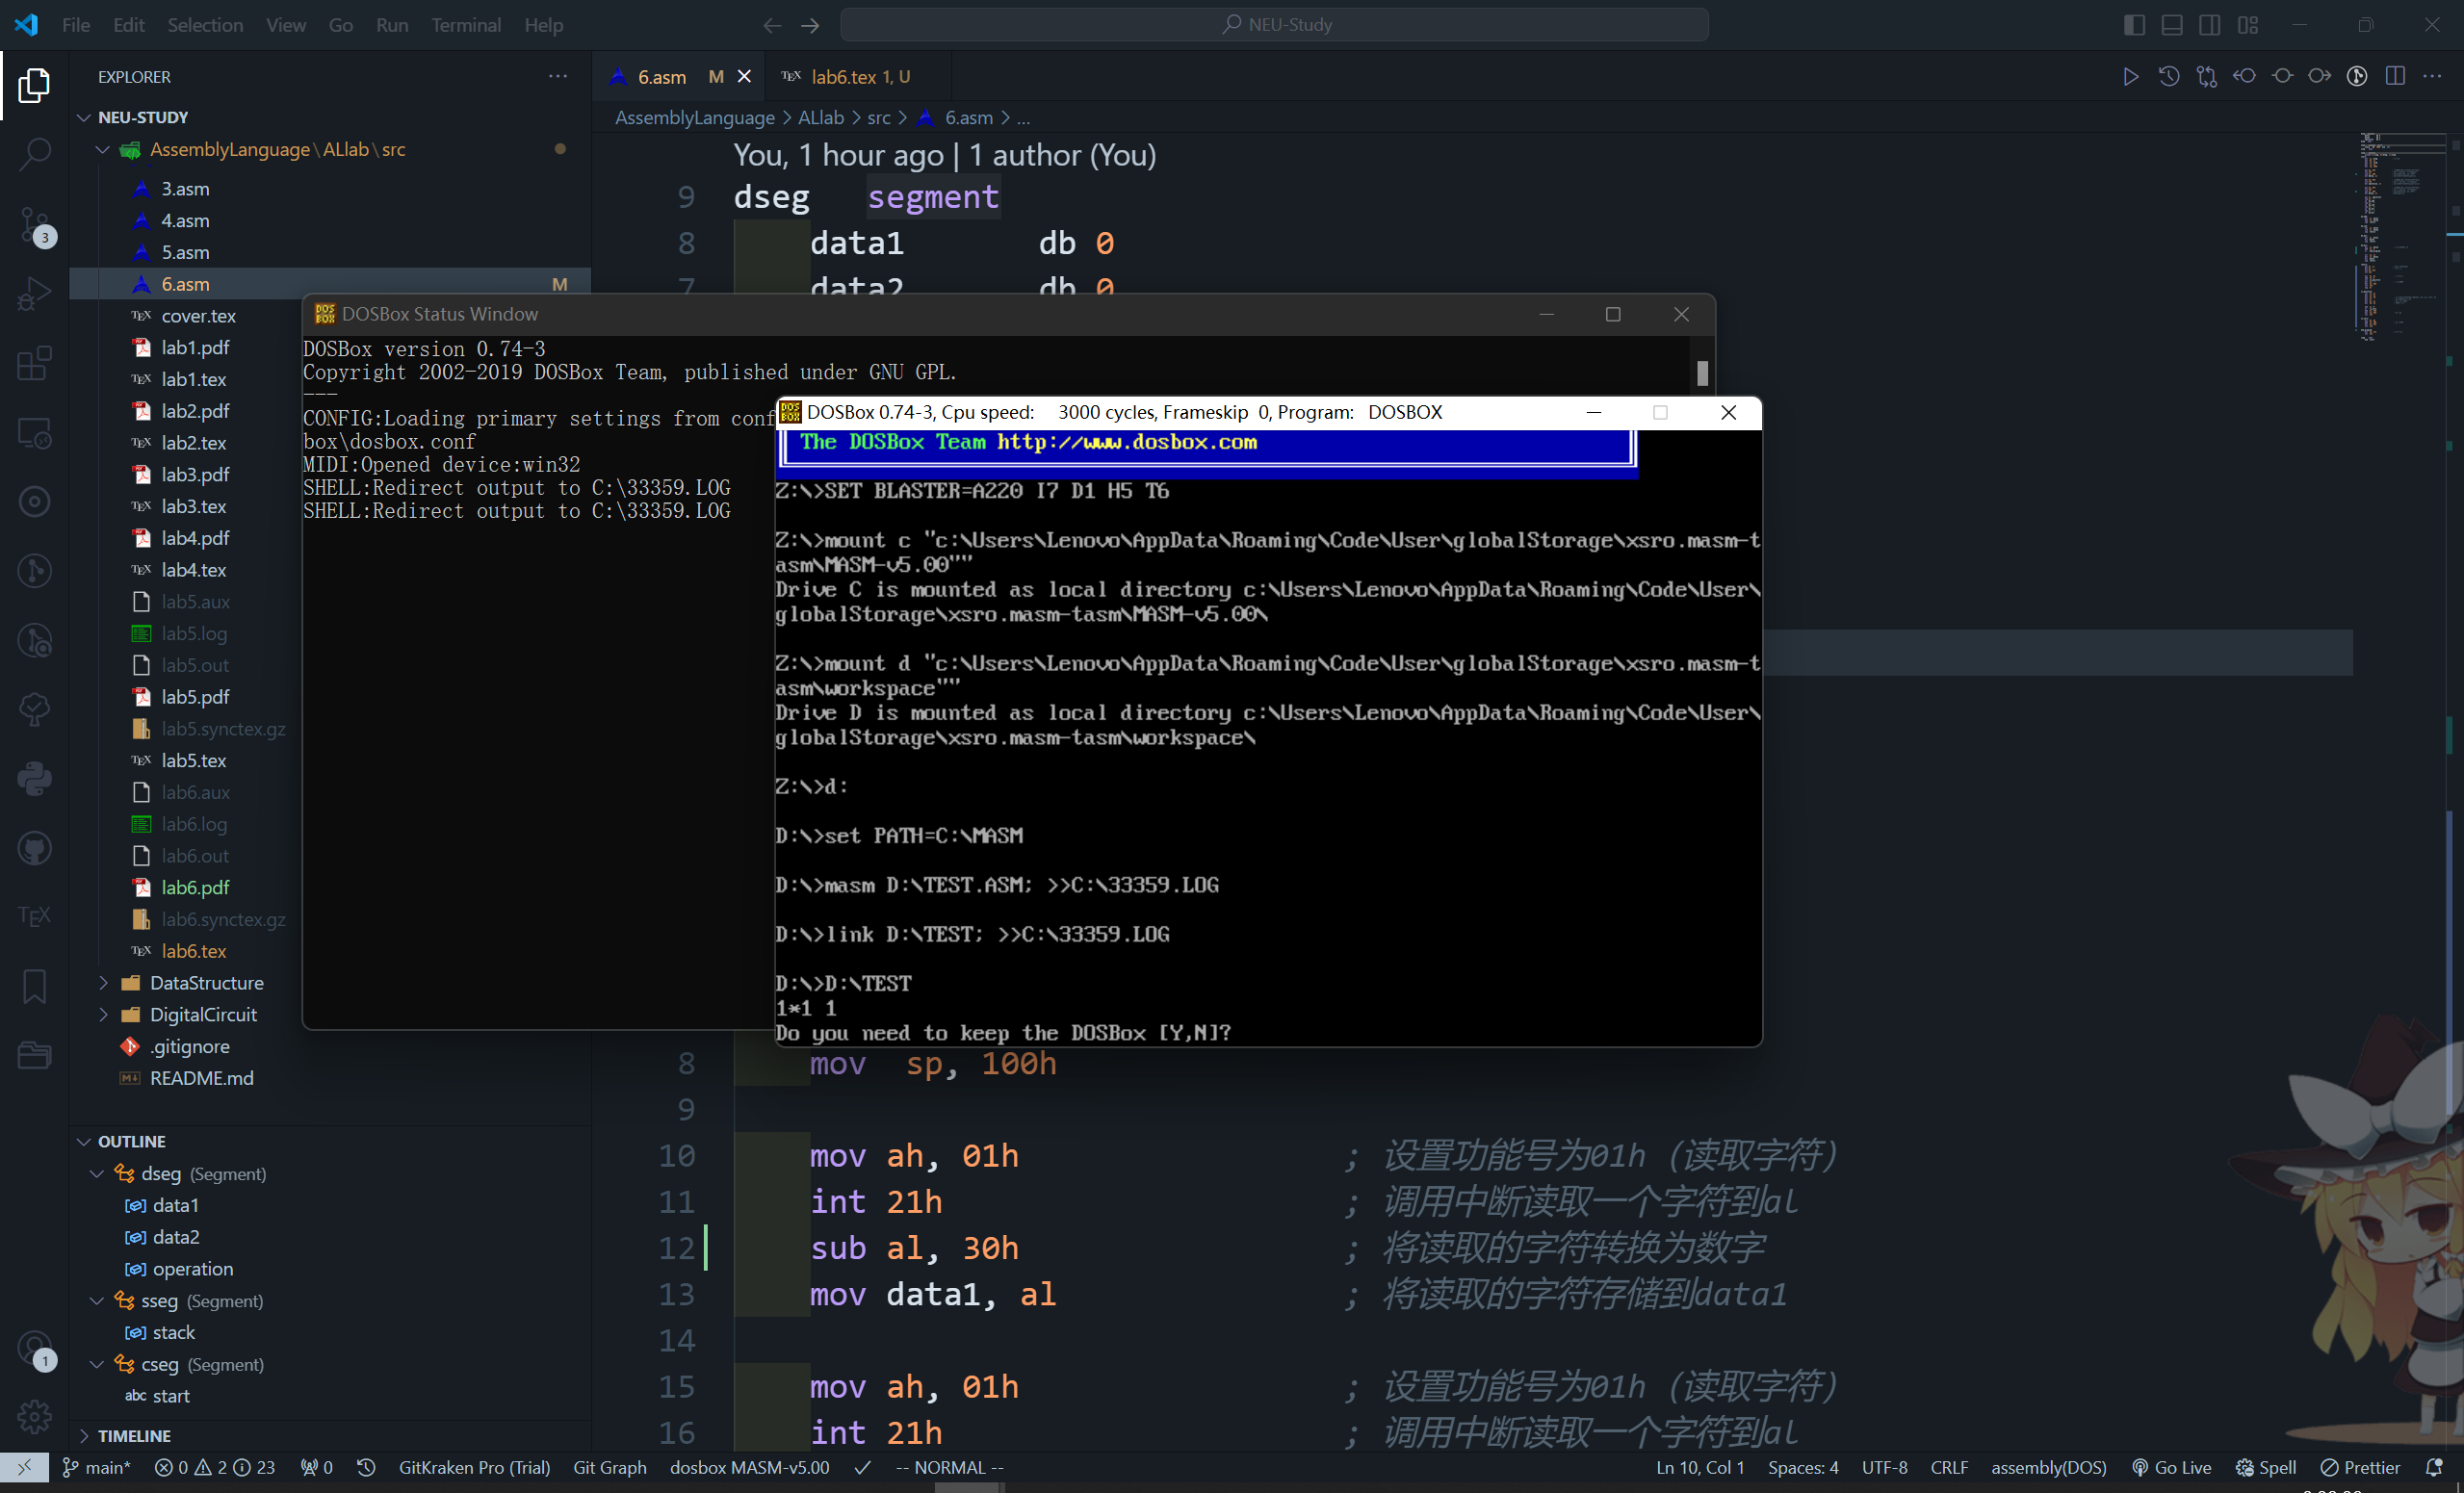
\includegraphics[width=1\textwidth]{image/AL_57.png}\end{center}
    \begin{center}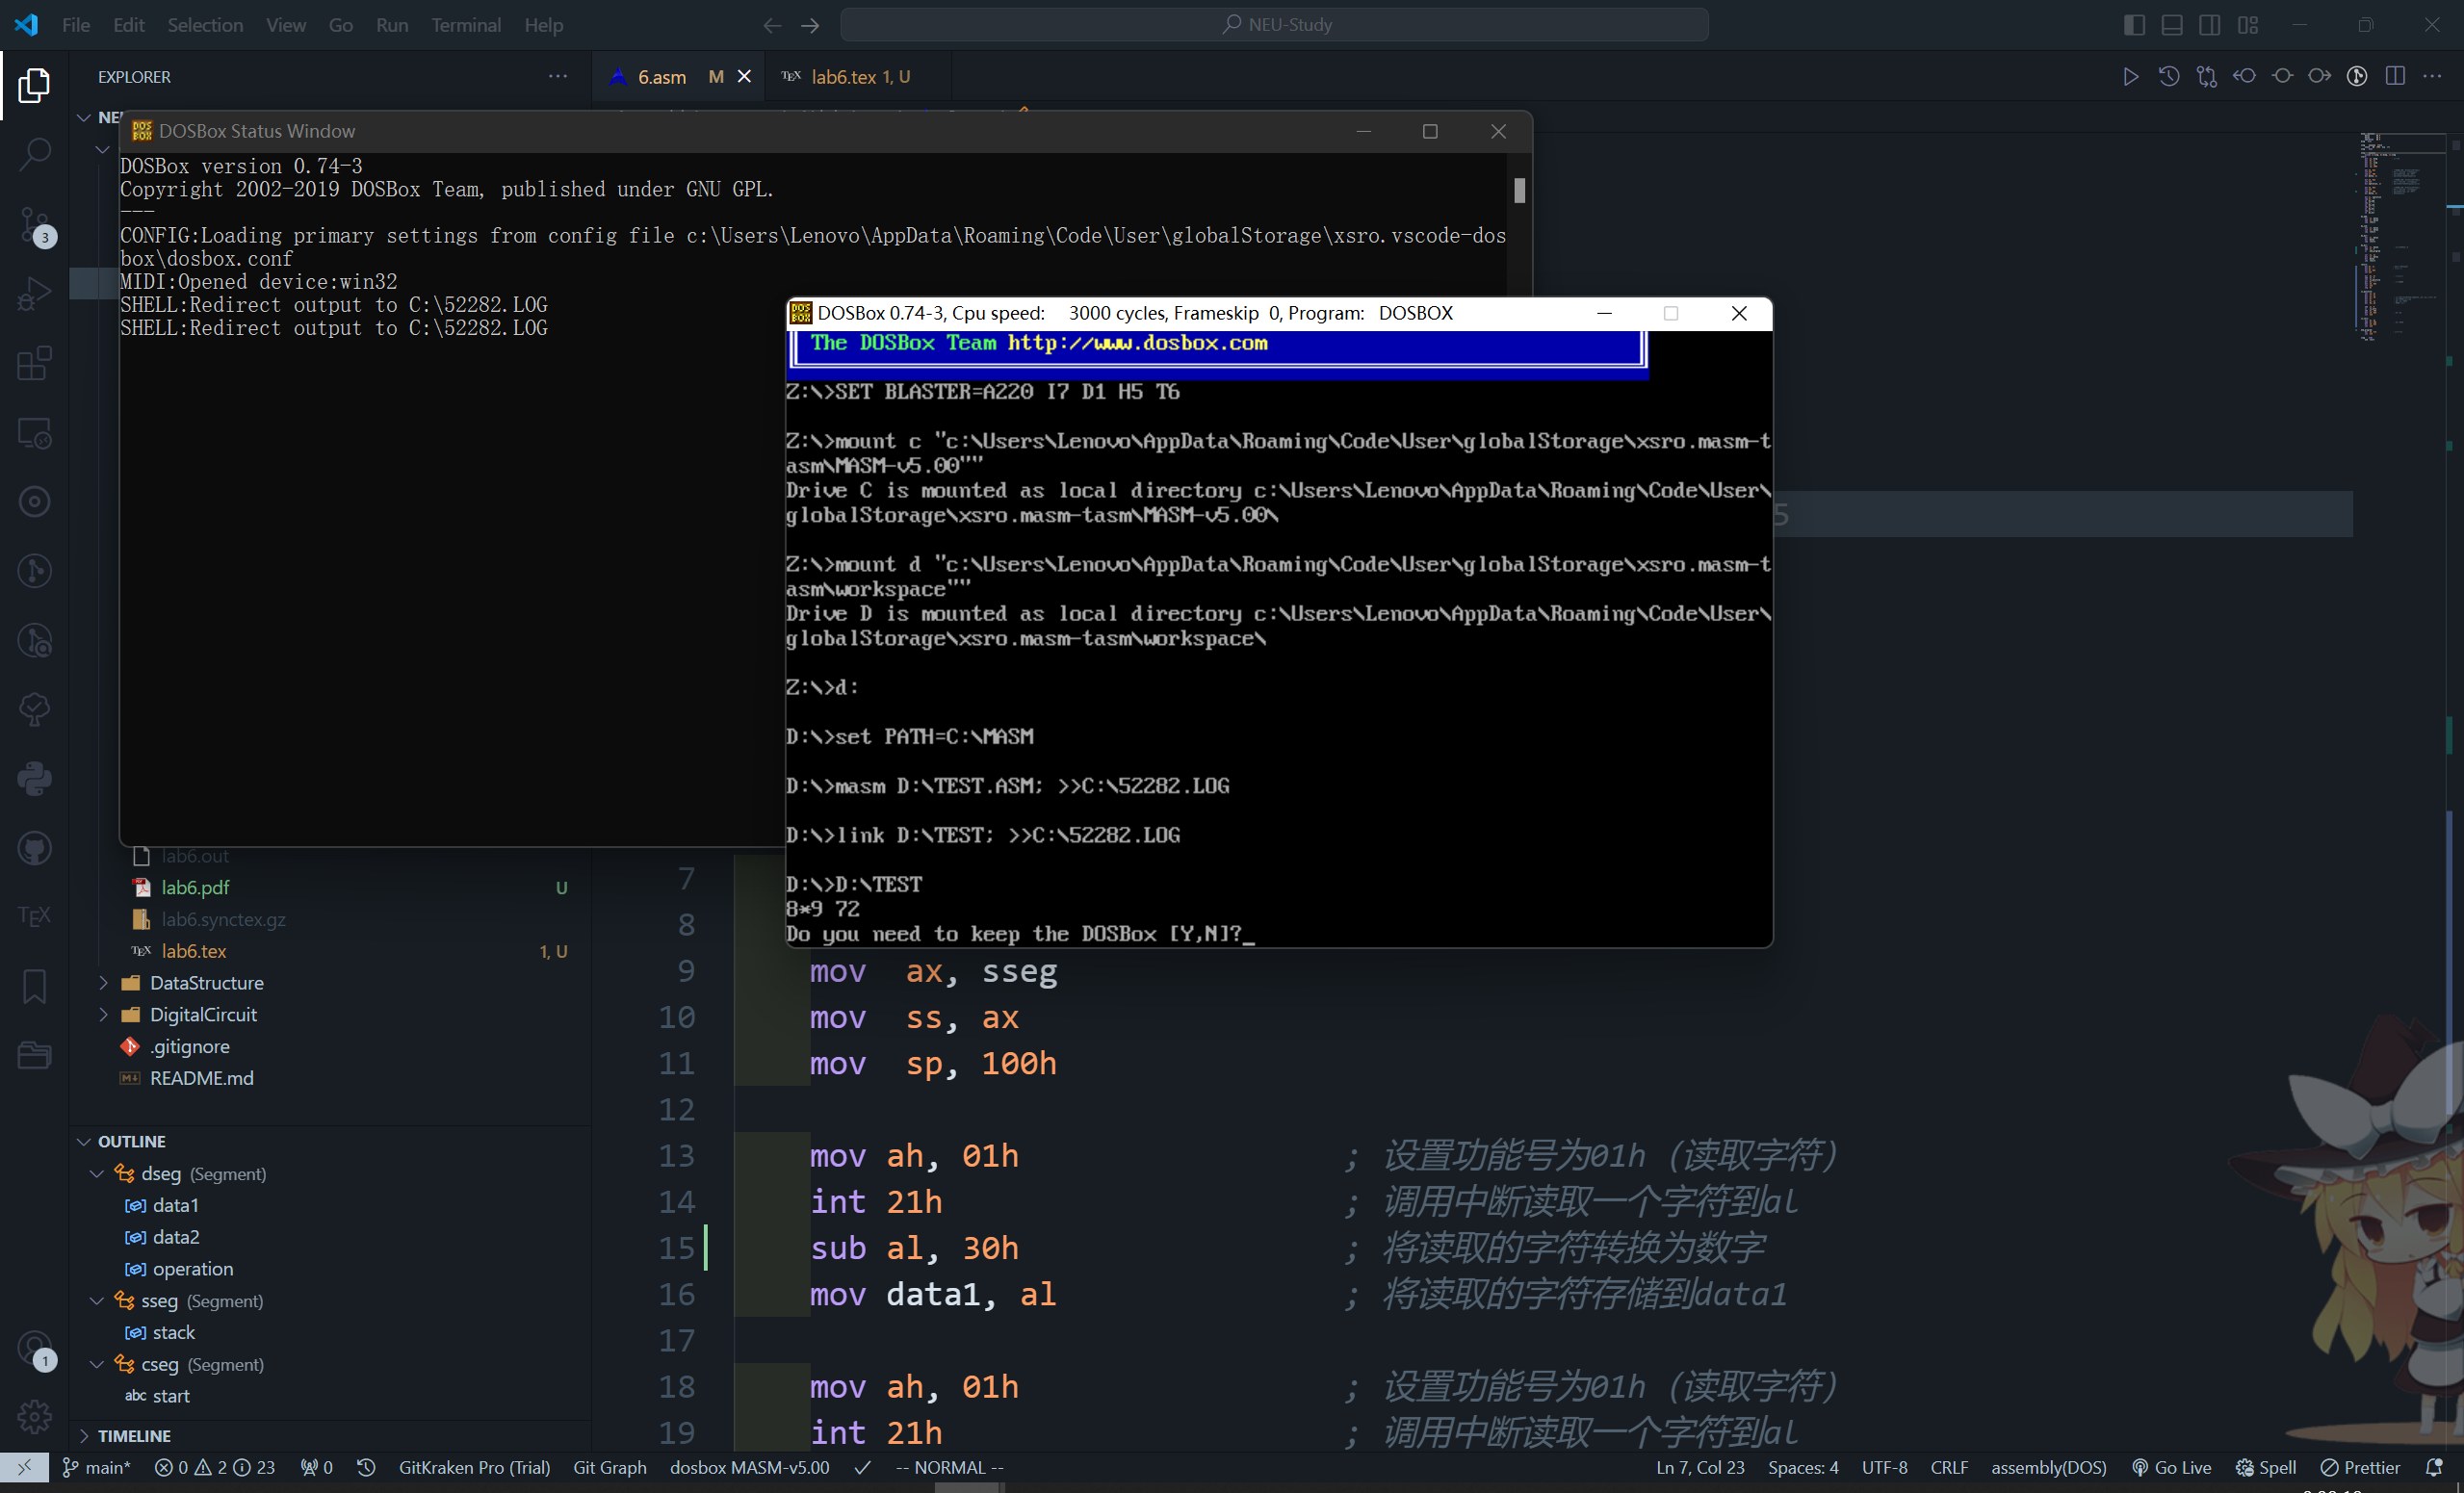
\includegraphics[width=1\textwidth]{image/AL_58.png}\end{center}
    除：
    \begin{center}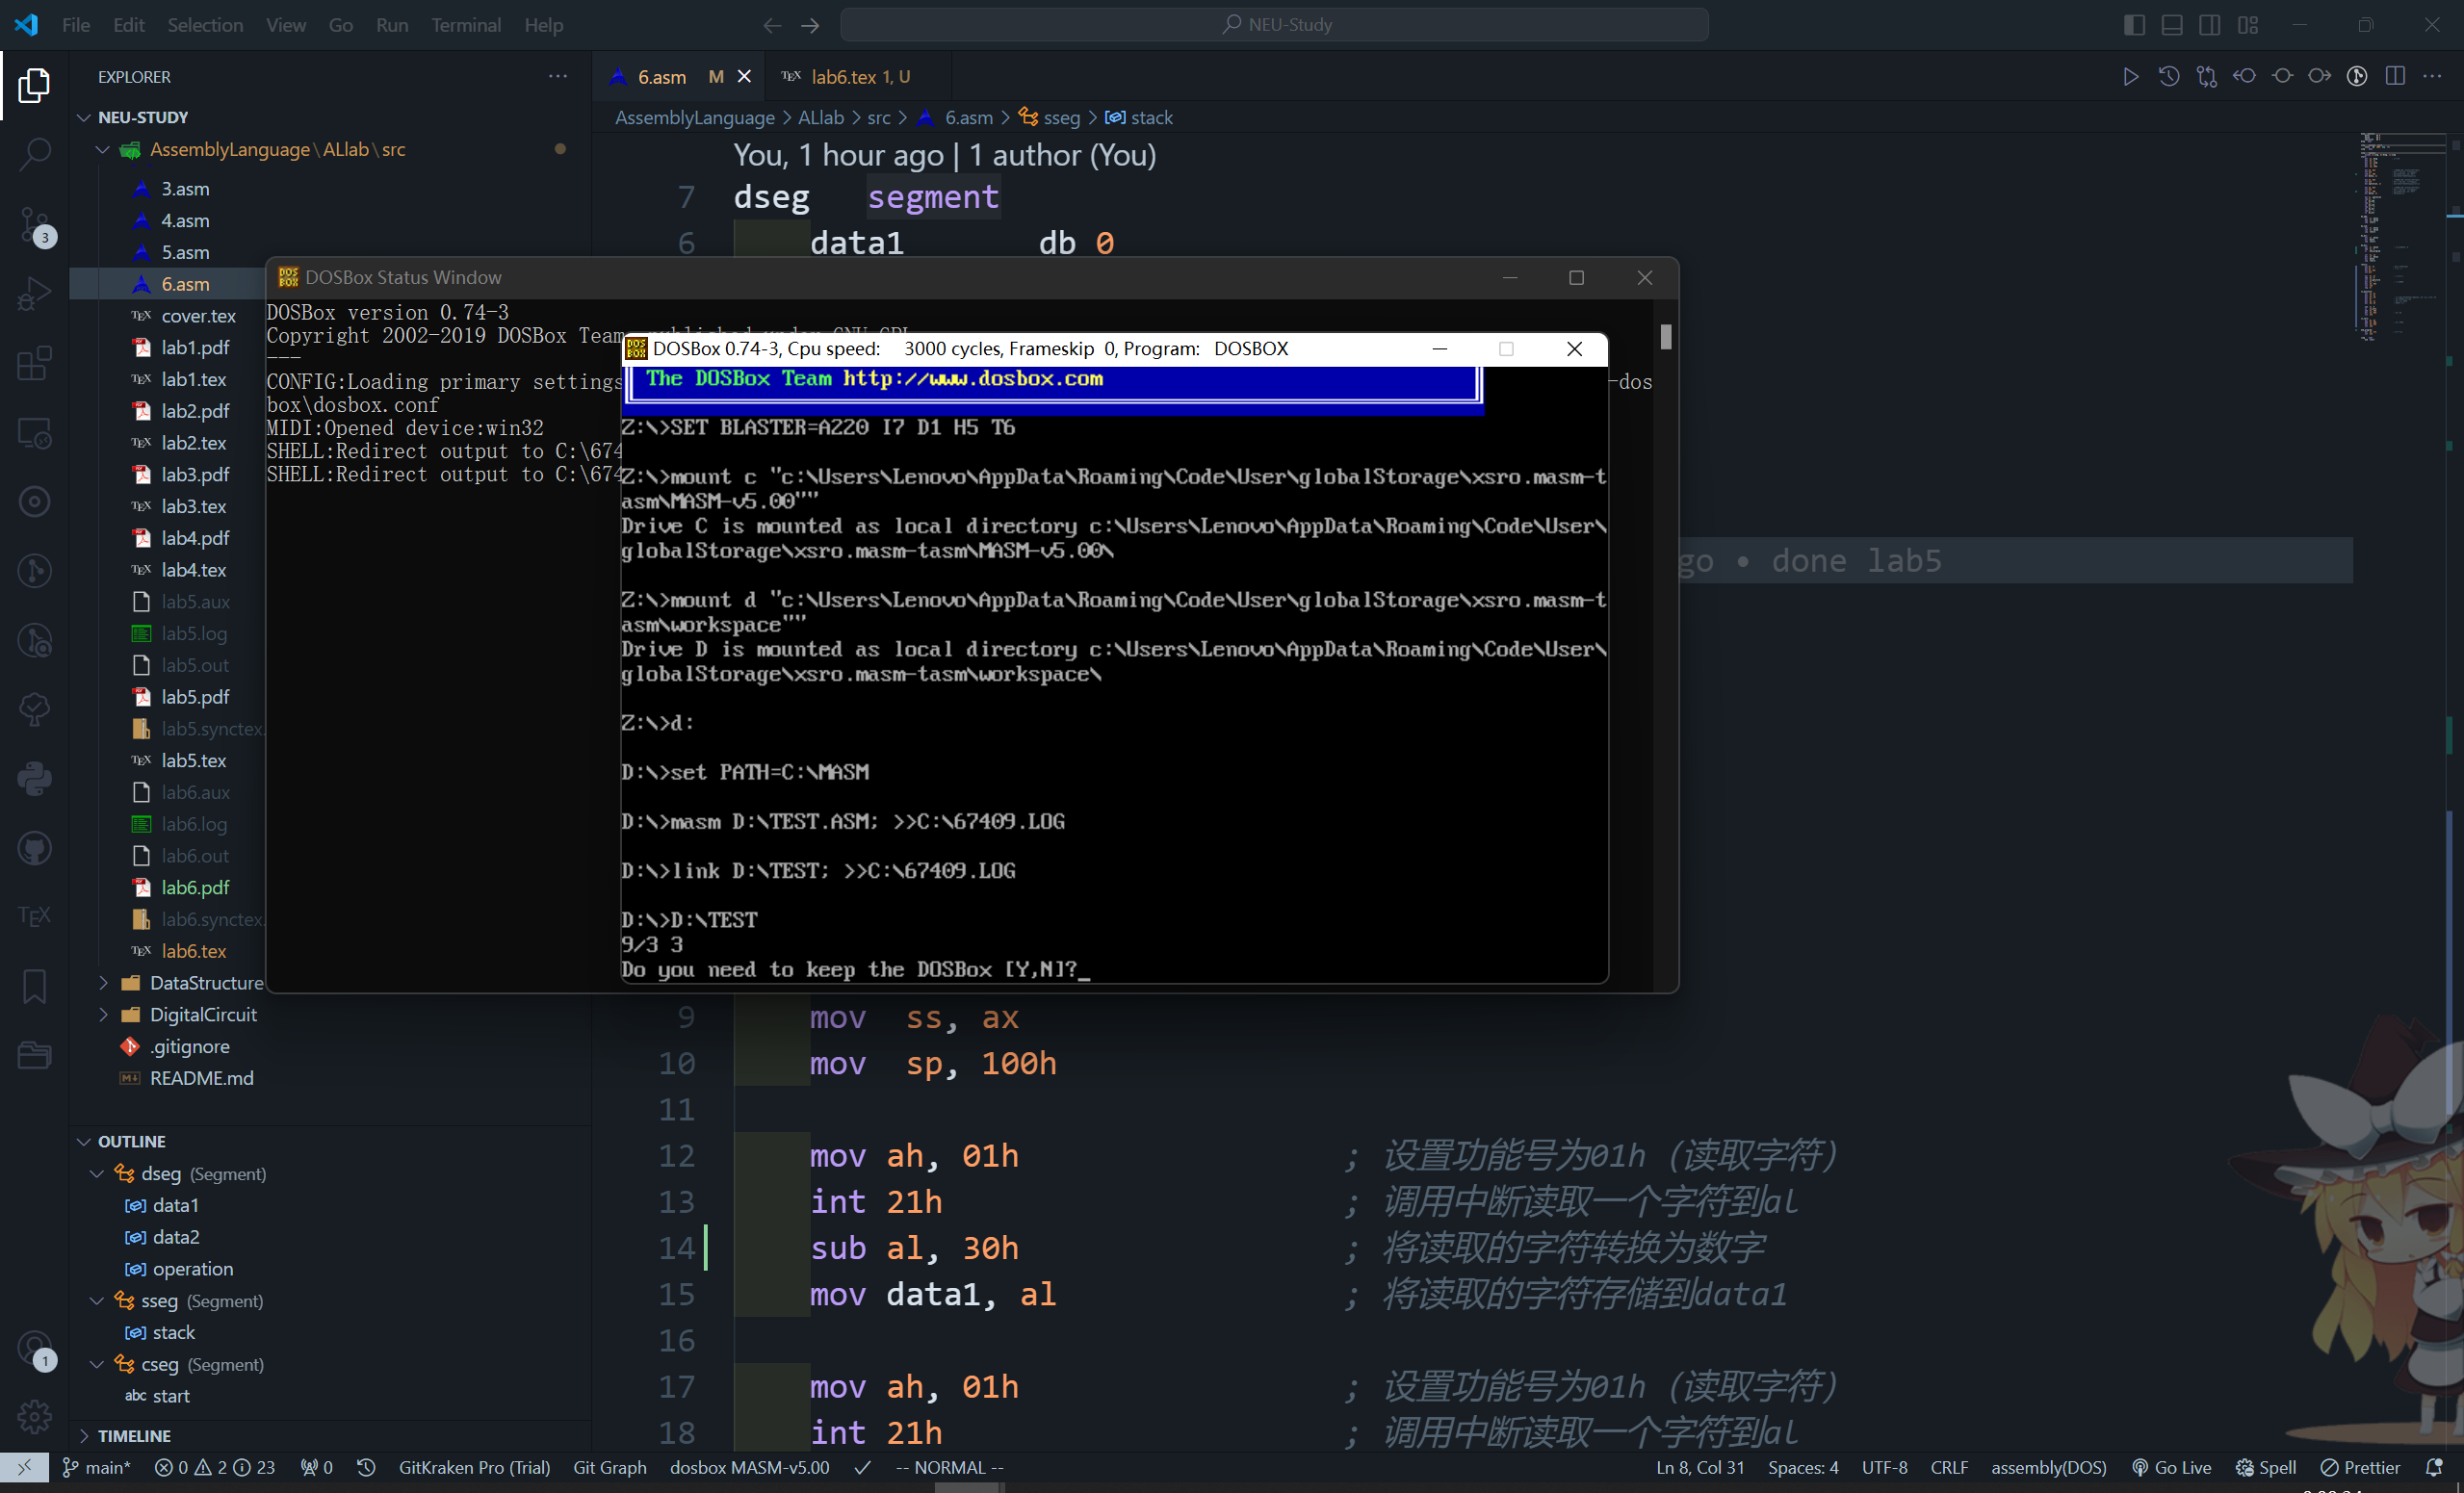
\includegraphics[width=1\textwidth]{image/AL_59.png}\end{center}
    \begin{center}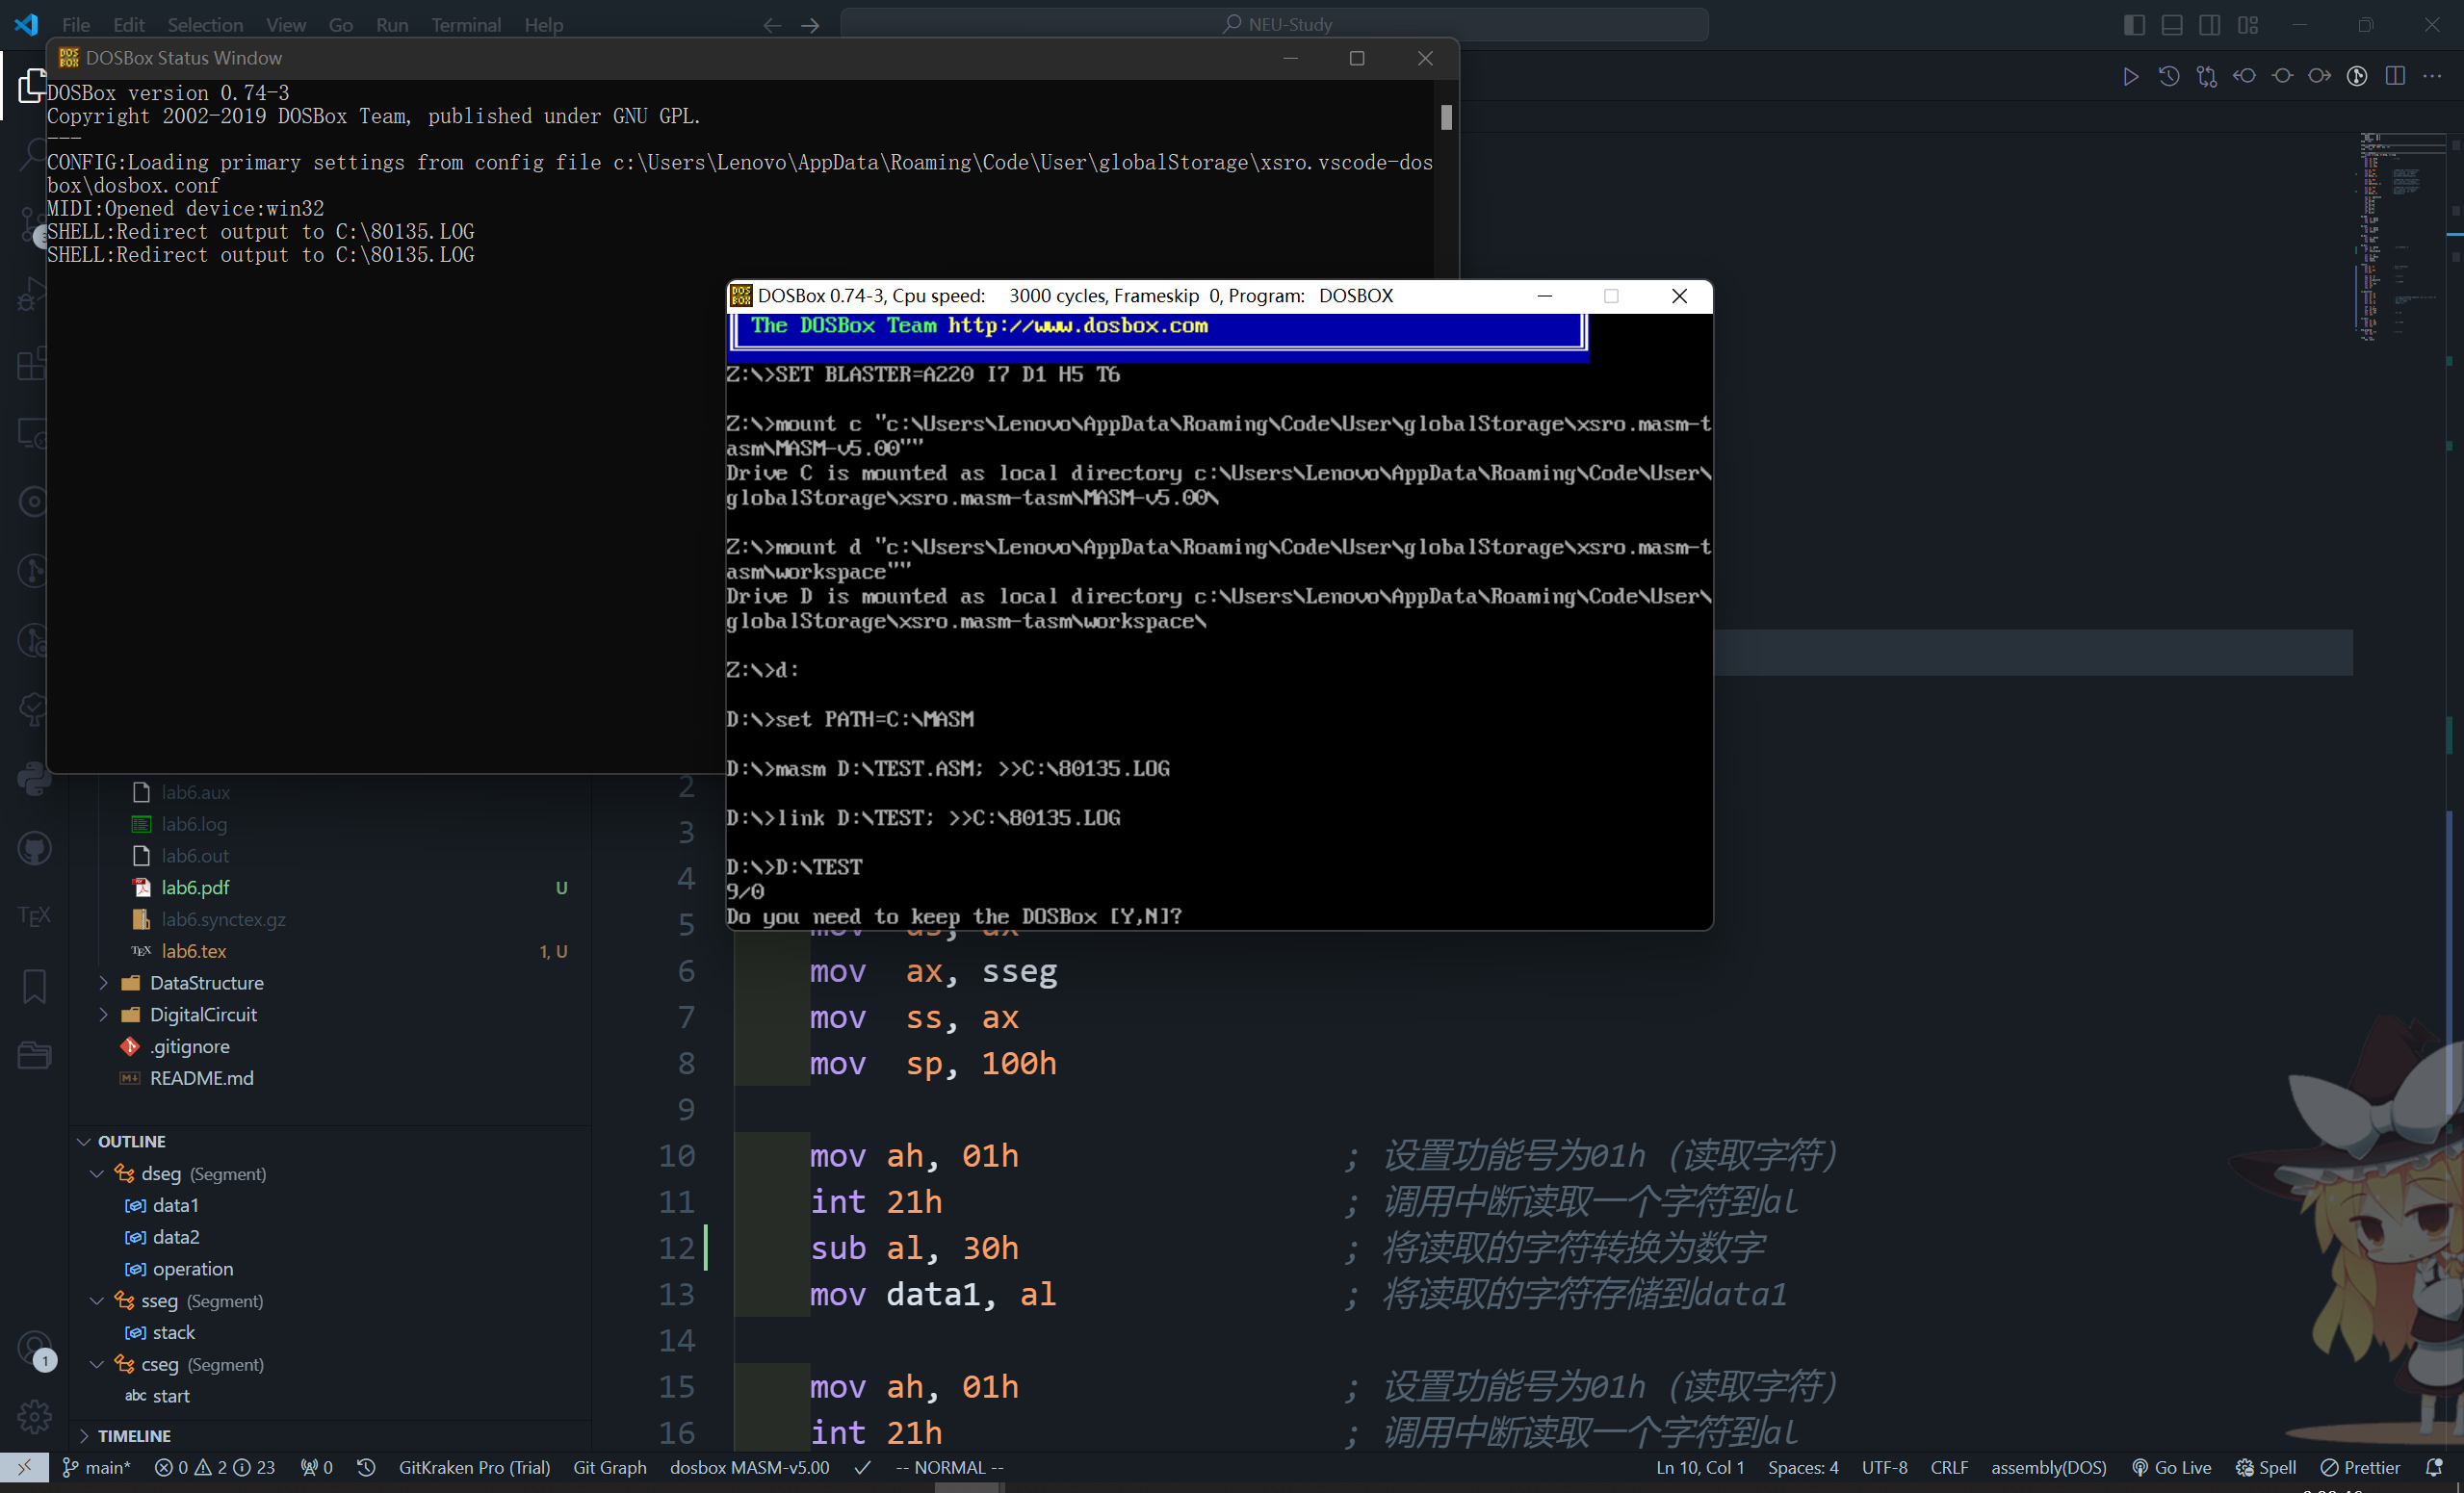
\includegraphics[width=1\textwidth]{image/AL_60.png}\end{center}
    
    被除数为0时，不输出数据。

    可见，程序能够正确地计算出加、减、乘、除的结果，并能够正确地处理负数和多位数的情况。
    \subsection{流程图}
    \begin{center}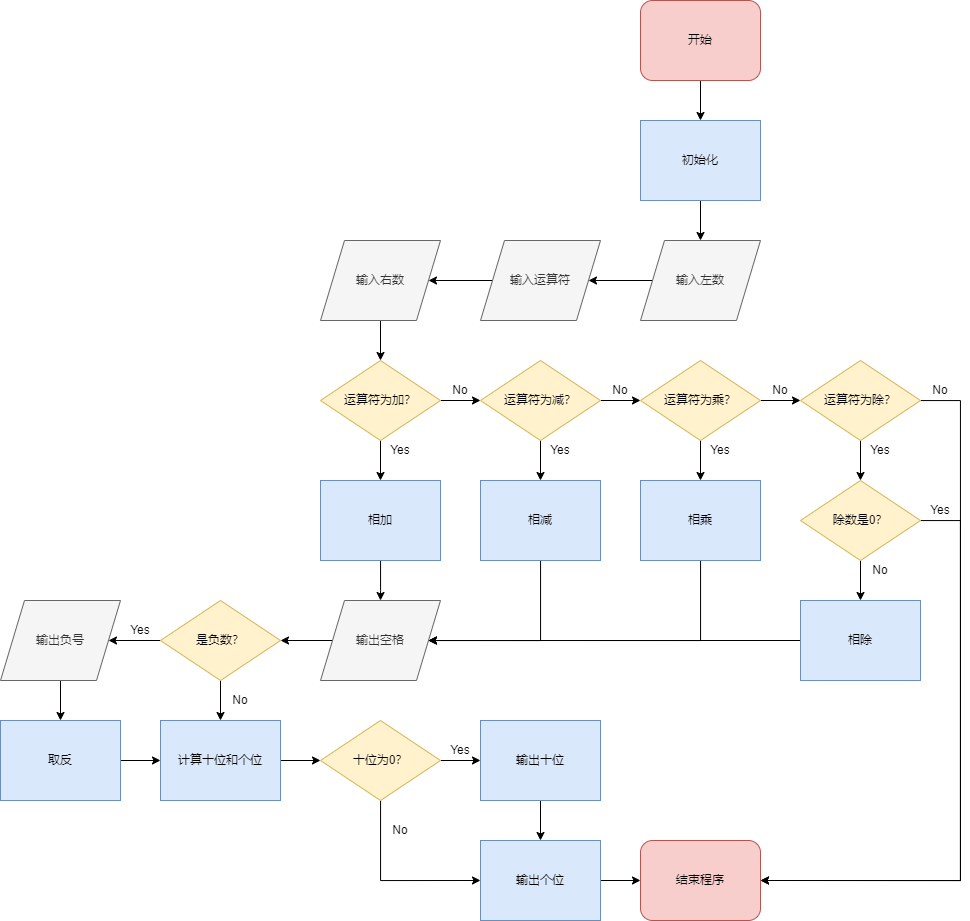
\includegraphics[width=1\textwidth]{image/AL_61.png}\end{center}

\section{心得体会}
通过这次实验，我对汇编语言的理解和应用能力有了显著的提升，特别是在处理基本算术运算和输入输出操作方面。
这次实验不仅加深了我对汇编语言指令的熟悉程度，也让我体会到了底层编程在精确控制计算机操作中的强大能力。

我学习了如何使用DOS中断（INT 21h）来进行键盘输入和屏幕输出，这是汇编语言中实现用户交互的基本方式。
通过实验，我掌握了字符与数字之间转换的方法，这对于处理用户输入尤为关键。
实现加、减、乘、除功能时，我使用了条件分支指令来选择不同的操作代码块，这加深了我对程序流程控制的理解。

最初，我直接将从键盘读入的字符用作数值计算，导致程序运行错误。
后来，我通过sub al, 30h指令将ASCII码转换为相应的数值，解决了这个问题。
在实现除法功能时，我最初忽略了除数为零的情况。这会导致程序运行时出错。
为了解决这个问题，我添加了对除数的检查，并在除数为零时通过特定流程安全退出程序。
在显示结果时，我需要考虑结果为负数和多位数的情况。
我通过添加检查结果符号的代码，并适当地调整输出格式，以确保所有结果都能正确显示。

这次实验使我对汇编语言有了更深入的了解，尤其是在如何利用汇编语言直接与硬件交互方面。
我也认识到了在编程时对细节的处理非常关键，特别是在底层编程中，每一个小错误都可能导致程序的不正常运行。
通过这次实验，我不仅提升了我的编程技能，也增强了我的问题解决能力和逻辑思维能力。
我期待将这些知识应用到更复杂的项目中，以解决更具挑战性的问题。

\begin{flushright}\begin{tabular}{rl}
    姓名: & 李俊洁\\
    班级: & 计算机2204 \\
    学号: & 20225443 \\
    课程: & 汇编语言程序设计 \\
    日期: & April 17, 2024 \\
    制作: & \LaTeX \\
    & 感谢您的批阅！
\end{tabular}\end{flushright}
\end{document}